%%%%%%%%%%%%%%%%%%%%%%%%%%%%%%%%%%%%%%%%%%%%%%%%%%%%%%%%%%%%%%%%%%%%%%%%%%%
%
%		Relazione del progetto di Peer-2-Peer
%
%				    Nicola Corti - 2014
%
%%%%%%%%%%%%%%%%%%%%%%%%%%%%%%%%%%%%%%%%%%%%%%%%%%%%%%%%%%%%%%%%%%%%%%%%%%%
\documentclass[a4paper,12pt]{article} 
\usepackage{graphicx}
\usepackage{vmargin}
\usepackage[italian]{babel} 
\usepackage[utf8x]{inputenc}
\usepackage{listings}
\usepackage{url}
\usepackage{pdflscape}
\usepackage{tabularx}
\usepackage{hyperref}
\usepackage{amsfonts}
\usepackage[usenames,dvipsnames,svgnames,table]{xcolor}

\usepackage{caption}
\usepackage{subcaption}

\usepackage{chngcntr}
\counterwithin{equation}{subsection}

\hyphenation{gossip}

\renewcommand\lstlistingname{Codice}
\addto\captionsitalian{\renewcommand\figurename{Immagine}}

%\setpapersize{A4}
%\setmarginsrb{15mm}{10mm}{15mm}{10mm}%
%             {0mm}{10mm}{0mm}{10mm}


\definecolor{LightLightGray}{RGB}{241,241,241}

\lstset{
basicstyle=\scriptsize\ttfamily,
keywordstyle=\color{MidnightBlue}\bfseries,
identifierstyle=\color{Black},
commentstyle=\color{Green}\itshape,
stringstyle=\color{Red}\ttfamily,
showstringspaces=false,
%numbers=left, numberstyle=\tiny,
%stepnumber=1, numbersep=10pt,
tabsize=4,
framexleftmargin=5mm, rulesepcolor=\color{LightLightGray},
frame=tb,
backgroundcolor=\color{LightLightGray},
language={Java},
%mathescape=true,
%fontadjust=true,
breaklines=true,breakatwhitespace=true,breakautoindent
}

\title{GOSSIPICO - Un approccio \emph{gossip-based} per la stima del numero dei nodi nelle reti dinamiche}
\author{Nicola Corti - 454413 \\Corso di Laurea Magistrale in Informatica - Universit\`a di Pisa}
\date{22 Aprile 2014}

 
\begin{document}
\maketitle

\begin{abstract}
Questa relazione ha lo scopo di illustrare l'algoritmo \textsc{gossipico}, un algoritmo gossip per il conteggio del numero dei nodi (o per altre funzioni di aggregazione) all'interno di una rete. \textsc{gossipico} ha in pi\`u, rispetto ad altri algoritmi di conteggio, un'elevata robustezza che lo rende adatto ad operare all'interno di reti che presentino un elevato grado di dinamicit\`a.
\end{abstract}

\tableofcontents

\section*{Introduzione}

Il conteggio del numero dei nodi di una rete \`e sempre stato uno dei problemi pi\`u affrontati quando si prendono in considerazione le reti decentralizzate, dove non \`e presente un nodo server che raccoglie le connessioni di tutti i client. In una rete di questo genere difficilmente ogni singolo nodo avr\`a la visione globale di tutti gli altri nodi della rete, in particolare se il numero dei nodi della rete diventa elevato.

Conoscere per\`o questo valore potrebbe essere comunque fondamentale per molte applicazioni che potrebbero ottimizzare i loro parametri di esecuzione (memoria da allocare, numero e frequenza dei messaggi da inviare, etc...).

Per effettuare questo genere di calcolo sono stati realizzati vari modelli con punti di forza e di debolezza differenti. Fra questi uno che merita di essere menzionato \`e il modello \emph{gossip}. Gli algoritmi \emph{gossip} effettuano fondamentalmente un continuo scambio di informazioni fra nodi ``vicini''\footnote{Per vicini non si intendono i nodi fisicamente vicini, ma i nodi appartenente al sottoinsieme dei nodi della rete noti al singolo peer} al fine di approssimare sempre pi\`u il numero dei nodi del sistema. I vari modelli di algoritmi, ed in particolare il modello \emph{gossip}, sono introdotti nella sezione \ref{sec:gossip}.

\textsc{gossipico} (presentato nella sezione \ref{sec:gossipico}) rappresenta un esempio di protocollo \emph{gossip} per il calcolo dei nodi di una rete. \textsc{gossipico} si basa fondamentalmente su due moduli che coesistono e funzionano in armonia al fine di velocizzare il calcolo: il modulo \textsc{count} (sezione \ref{sec:count}) si occupa di effettuare il conteggio vero e proprio, conservando in ogni nodo le informazioni sull'approssimazione finora raggiunta dall'algoritmo, mentre il modulo \textsc{beacon} (sezione \ref{sec:beacon}) si occupa di individuare in modo casuale dei nodi di riferimento (detti appunti nodi \emph{beacon}) verso cui veicolare i messaggi al fine di velocizzare il processo di conteggio.

Uno dei punti di forza di \textsc{gossipico} sta nel fatto che l'algoritmo si adatta molto bene a reti che sono dinamiche, con nodi che si connettono e si disconnettono nel tempo. Gli algoritmi di conteggio classici presentano infatti delle criticit\`a nel caso in cui un nodo si disconnetta dalla rete. Un ulteriore scenario si presenta se la disconnessione di un singolo nodo porta alla disconnessione dell'intera rete in due componenti distinte. \textsc{gossipico} affronta queste difficolt\`a tramite alcune accortezze (sezione \ref{sec:dynamic}) che gli permettono di affrontare senza troppe difficolt\`a i conteggi su reti dinamiche.

Per poter valutare le performance dell'algoritmo \`e stato realizzata un'implementazione dell'algoritmo utilizzando il simulatore PeerSim (\cite{rif2}). \`E possibile conoscere i comandi necessari per far funzionare la simulazione leggendo la user guide (sezione \ref{sec:guide}) mentre i risultati delle simulazioni su varie tipologie di rete sono raccolti nella sezione perfomance (sezione \ref{sec:performance}).

\section{Gli algoritmi \emph{gossip-based}}
\label{sec:gossip}

Alcune delle operazioni che potrebbero risultare banali in una rete organizzata con un paradigma \emph{client-server} possono presentare alcune criticit\`a se considerate all'interno di una rete \emph{peer-to-peer}.

Il conteggio del numero dei nodi risulta essere una delle prime, ma si pensi anche alla distribuzione di un'informazione a tutti i nodi della rete (ad esempio una nuova release di un software), oppure al recupero di informazioni sullo stato globale dei nodi stessi (quanti nodi si sono disconnessi, etc...). In questo contesto risulta necessario disporre di algoritmi che siano scalabili, efficienti e che al contempo non basino il loro funzionamento su un nodo centrale che potrebbe disconnettersi improvvisamente.

\`E in questo contesto che sono nati gli algoritmi \emph{gossip} anche detti algoritmi \emph{epidemici}. 

Per comprendere il principio che fonda le basi di questa classe di algoritmi si pensi al modo con cui si propagano i pettegolezzi in un gruppo di persone oppure al modo con cui si propaga un'infezione virale: casualmente un soggetto infettato incontra un altro soggetto suscettibile e lo infetta.

Risulta chiaro come questo meccanismo porti a lungo termine ad uno stato in cui tutti i soggetti sono infettati, ovvero tutti i nodi hanno raccolto l'informazione presente nella rete.

Ogni soggetto pu\`o trovarsi in una serie di stati differenti e transire verso un altro stato in base a come interagisce con gli altri nodi e con l'informazione:
\begin{description}
\item[\emph{susceptible}] Rappresenta un soggetto che non \`e ancora stato  coinvolto dall'informazione,
\item[\emph{infected}] Rappresenta un soggetto che \`e stato coinvolto e che sta diffondendo l'informazione,
\item[\emph{recovered}] Rappresenta un soggetto che non \`e pi\`u interessato a diffondere l'informazione.
\end{description}

Inoltre in base a come vengono svolte le comunicazioni si possono individuare protocollo di tipo differente:
\begin{description}
\item[push] Il soggetto che ha stabilito la comunicazione invia l'informazione che sta mantenendo,
\item[pull] Il soggetto che ha stabilito la comunicazione raccoglie l'informazione dal soggetto che ha contattato,
\item[push/pull] Il soggetto che ha stabilito la comunicazione scambia le proprie informazioni con il soggetto che ha contattato.
\end{description}

\subsection{Algoritmi per il conteggio dei nodi}

In passato sono stati presentati altri modelli per il conteggio dei nodi di una rete, in particolare si possono raggruppare i modelli proposti fra:
\begin{itemize}
\item Algoritmi basati su \emph{probabilistic polling}, che stimano la dimensione della rete in base alla risposta ad una richiesta inviata da un nodo,
\item Algoritmi basati sul \emph{random walk}, che stimano la dimensione della rete in base al numero di archi percorsi da un messaggio che segue un percorso casuale fra i nodi,
\item Algoritmi basati sul \emph{gossip}, in cui ogni nodo possiede una valore e si procede ad approssimare il conteggio effettuando delle medie fra i valori ad iterazioni successive.
\end{itemize}

\textsc{gossipico} rappresenta un esempio di algoritmo appartenente a quest'ultima classe, offrendo per\`o il meccanismo \textsc{beacon} per velocizzare il calcolo della stima.
\section{GOSSIPICO}
\label{sec:gossipico}

L'algoritmo \textsc{gossipico} (\cite{rif1}) nasce presso l'Universit\`a di Delft con lo scopo primario di realizzare un algoritmo \emph{gossip-based} che permetta di realizzare il calcolo di funzioni di aggregazione su reti decentralizzate. Il protocollo originariamente presentato in \cite{rif1} permette di effettuare solamente il calcolo dei nodi, ma pu\`o essere facilmente esteso permettendo il calcolo di altre funzioni di aggregazione (in particolare della somma, del massimo, del minimo e della media).

\textsc{gossipico} \`e formato da due moduli:
\begin{description}
\item[COUNT] Che effettua la fase di conteggio vera e propria. Si occupa di raccogliere i messaggi e di ``combinarli'' fra di loro al fine di portare la rete verso lo stato di convergenza.
\item[BEACON] Permette di velocizzare la fase di \textsc{count}, in particolare organizzando la rete in eserciti (\emph{Army}) che si combattono al fine di determinare un unico vincitore. In questo modo i messaggi della rete saranno veicolati verso il vincitore che si occuper\`a di svolgere il ruolo di raccolta dell'informazione globale.
\end{description}

Si noti che il modulo di \textsc{count} potrebbe funzionare anche in modalit\`a \emph{stand-alone}, ma il modulo di \textsc{beacon} velocizza notevolmente il calcolo (vedi sezione \ref{sec:performance}).

L'algoritmo \`e stato implementato tramite il simulatore Peersim utilizzando un insieme di classi che verranno presentate nel seguito e che sono sintetizzate nel seguente diagramma delle classi (immagine \ref{img:uml}). Si noti che non sono presenti tutti gli attributi e tutti i metodi delle classi poich\'e sono stati rappresentati solamente i pi\`u significativi al fine di non appesantire troppo la rappresentazione.

\begin{figure}[ht]
\centering
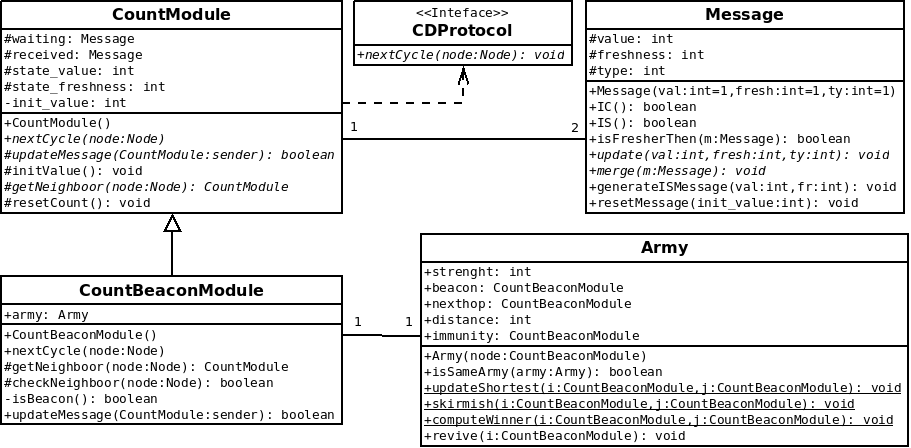
\includegraphics[height=6cm]{uml.png}
\caption{Diagramma delle classi realizzate}
\label{img:uml}
\end{figure}

Le classi sono state realizzate implementato l'interfaccia \textsf{CDProtocol}, ovvero un protocollo Peersim che procede a cicli successivi. \textsf{CDProtocol} rappresenta una delle due interfacce offerte da Peersim per implementare un protocollo, insieme all'interfaccia \textsf{EDProtocol} (protocollo che funziona tramite eventi); si \`e scelta la prima interfaccia in quanto risulta pi\`u naturale nell'implementare l'algoritmo \textsc{gossipico} poich\'e si dispone della descrizione del comportamento ciclo per ciclo.

\section{Il modulo COUNT}
\label{sec:count}

Il modulo \textsc{count} \`e realizzato dalla classe \textsf{CountModule} che esegue ad ogni ciclo la seguente computazione:
\begin{enumerate}
\item Contatta uno dei vicini scelto casualmente,
\item Invia il proprio messaggio in attesa,
\item Genera un nuovo messaggio contenente l'informazione finora raccolta.
\end{enumerate}

Quando invece un nodo riceve un messaggio in input, esso aggiorna il proprio messaggio in attesa in funzione del messaggio appena ricevuto.

Per comprendere a fondo il funzionamento di \textsc{count} risulta per\`o necessario conoscere la struttura dei messaggi inviati e ricevuti da ogni nodo.

\subsection{Struttura dei messaggi}

Ogni nodo durante tutto il calcolo riceve ed invia costantemente messaggi che hanno la seguente struttura
$$ < C, F, T > $$
\begin{description}
\item[$C \in \mathbb{Z}$] Rappresenta il valore attualmente contenuto del messaggio, ovvero l'approssimazione che finora \`e stata calcolata
\item[$F \in \mathbb{N}$] Indica quanto \`e recente l'informazione contenuta nel messaggio, a freschezza maggiore corrisponde un messaggio pi\`u recente
\item[$T \in \{0,1\}$] Rappresenta il tipo del messaggio che pu\`o essere di \emph{Information Spreading} (IS, $T = 0$) oppure di \emph{Information Collecting} (IC, $T = 1$).
\end{description}
In particolare il tipo del messaggio rappresenta la natura dell'informazione contenuta al suo interno:
\begin{description}
\item[IS] Indica un messaggio che sta diffondendo informazioni sulla rete. In particolare ogni nodo periodicamente genera un messaggio di tipo IS, al fine di informare la rete del dato che finora ha raccolto,
\item[IC] Indica un messaggio che contiene dell'informazione che deve essere ancora raccolta. I nodi della rete daranno maggiore priorit\`a a questi messaggi rispetto ai messaggi IS. Quando due messaggi IC si incontrano essi verranno combinati al fine di accumulare sempre pi\`u informazione.
\end{description}
La computazione comincia inizializzando tutti i nodi della rete con messaggi formati nel modo seguente $\{ 1, 1, 1 \}$\footnote{Questa inizializzazione vale solamente per il caso in cui si effettui il conteggio dei nodi}. I messaggi inizieranno a fluire nella rete ed i messaggi IC che si incontrano verranno combinati, fin quando non si sar\`a raccolta tutta l'informazione presso un singolo nodo, avendo dunque un solo messaggio IC.


\subsection{Regole di \emph{message-combining}}
\label{sec:combining}

Ogni nodo conserva al proprio interno uno stato formato da:
\begin{description}
\item[$M_r$] Ovvero il messaggio appena ricevuto dal peer. I nodi utilizzano $M_r$ per conservare il messaggio appena ricevuto e lo confrontano insieme al messaggio in attesa ($M_w$) per calcolare un nuovo messaggio in attesa.
\item[$M_w$] Ovvero il messaggio in attesa. Ogni nodo invia nel proprio ciclo di esecuzione il messaggio $M_w$ ad un altro nodo vicino scelto in modo casuale.
\item[$C_s$] Rappresenta il valore attualmente conservato dallo stato del nodo.
\item[$F_s$] Rappresenta la freschezza pi\`u alta attualmente vista dal nodo.
\end{description}

Dopo ogni invio un nodo utilizza i valori $C_s$ e $F_s$ per generare un nuovo messaggio $\{ C_s, F_s, 0 \}$ generando dunque un messaggio di tipo IS per informare la rete sull'informazione finora raccolta.

Quando un nodo riceve un messaggio, confronta i messaggi $M_r$ e $M_w$ utilizzando le seguenti regole:
\begin{itemize}
\item $M_r.Tipo$ = IS e $M_w.Tipo$ = IS, si aggiorna $M_w$ al messaggio che contiene il valore di $Freschezza$ pi\`u elevato,
\item $M_r.Tipo$ = IC e $M_w.Tipo$ = IS, si da priorit\`a all'informazione contenuta dentro il messaggio IC, per cui si imposta $M_w \leftarrow M_r$,
\item $M_r.Tipo$ = IS e $M_w.Tipo$ = IC, si da sempre priorit\`a all'informazione contenuta dentro il messaggio IC, per cui si scarta il messaggio $M_r$,
\item $M_r.Tipo$ = IC e $M_w.Tipo$ = IC, in questo caso si effettua il \emph{combining} fra i due messaggi IC al fine di generare un nuovo messaggio IC formato nel modo seguente $$\{ M_r.C + M_w.C, M_r.F + M_w.F, 1 \}$$
\end{itemize}
Contestualmente a queste operazioni, il nodo che riceve un messaggio provvede anche ad aggiornare i propri valori $C_s$ e $F_s$ in modo da mantenere le proprie informazioni le pi\`u aggiornate possibile.

Grazie a questo meccanismo il numero totale dei messaggi IC all'interno della rete tende a decrescere fino ad arrivare ad un singolo messaggio che conterr\`a l'informazione aggregata.

Le variabili $C_s$ e $F_s$ sono necessarie in quanto il nodo ad ogni ciclo di esecuzione, dopo aver inviato il proprio messaggio in attesa, generer\`a un nuovo messaggio in attesa di tipo IS partendo dalle informazioni sullo stato, che verr\`a inviato al ciclo successivo per informare la rete sulle informazioni da lui raccolte finora.

\subsection{Implementazione}

\begin{figure}[ht]
\centering
\begin{subfigure}[b]{1\textwidth}
	\centering
	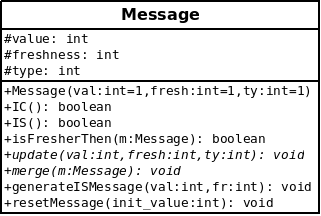
\includegraphics[height=4cm]{message_uml.png}
	\caption{Classe \textsf{Message}}
	\label{img:message_uml}
	\vspace{0.5cm}
\end{subfigure}
\begin{subfigure}[b]{1\textwidth}
	\centering
	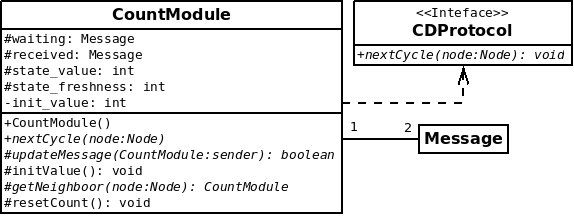
\includegraphics[height=4cm]{count_uml.png}
	\caption{Classe \textsf{CountBeacon}}
	\label{img:count_uml}
\end{subfigure}
\caption{Diagramma delle classi relative al modulo \textsc{count}}
\end{figure}

I messaggi sono realizzati dalla classe \textsf{Message} che dispone di tutti i metodi per la gestione dei messaggi (immagine \ref{img:message_uml}), mentre il modulo \textsc{count} \`e realizzato dalla classe \textsf{CountModule} (immagine \ref{img:count_uml}).

In particolare la classe \textsf{Message}, oltre ad una serie di costruttori base, offre i metodi \textsf{IC()} ed \textsf{IS()} per verificare il tipo di un messaggio, \textsf{isFresherThen()} per confrontare la freschezza, \textsf{update(val, fresh, ty)} per aggiornare tutti i campi di un messaggio (usato per l'invio di messaggi), \textsf{merge(m)} per calcolare la combinazione di due messaggi, \textsf{generateISMessage(val, fr)} per generare un nuovo messaggio IS e il metodo \textsf{reset(val)} per reimpostare il valore di un messaggio.

La classe \textsf{CountModule} dispone di due field di tipo \textsf{Message} che rappresentano rispettivamente i messaggi $M_w$ e $M_r$, dispone inoltre delle variabili dello stato $C_s$ e $F_s$.

Per quanto riguarda i metodi, la classe \textsf{CountModule} implementa il metodo \textsf{nextCycle(node)} come richiesto dall'interfaccia \textsf{CDProtocol} di Peersim, in cui \`e presente tutta la logica del singolo nodo. Sono presenti inoltre altre funzioni di comodo quali:
\begin{description}
\item[\textsf{updateMessage(sender)}] Per aggiornare il messaggio $M_w$ in base alle regole descritte nella sezione \ref{sec:combining},
\item[\textsf{initValue()}] Per impostare il valore iniziale $C_i$ con cui iniziare il calcolo,
\item[\textsf{getNeighboor()}] Per scegliere in modo casuale un vicino dalla rete offerta da Peersim e configurata nel file di configurazione,
\item[\textsf{resetCount()}] Per riportare il messaggio $M_w$ allo stato iniziale.
\end{description}

Si faccia particolare attenzione anche al metodo \textsf{clone()}, override dalla classe \textsf{Object}, in quanto Peersim utilizza questo metodo per generare nuove istanze dei singoli protocolli.

\section{Il modulo BEACON}
\label{sec:beacon}

\textsc{gossipico} prevede che oltre al modulo \textsc{count} sia presente anche un modulo \textsc{beacon}. Il modulo \textsc{beacon} serve per ``guidare'' i nodi nell'invio dei messaggi IC verso un nodo unico (che si chiamer\`a appunto \emph{beacon}, dall'inglese faro) in modo da velocizzare il processo di \emph{message-combining} dei messaggi che raccolgono l'informazione.

Si pensi al caso in cui nella rete rimangono solamente due messaggi di tipo IC: la convergenza viene raggiunta quando i due messaggi si incontrano presso uno stesso nodo. Il tempo necessario per raggiungere questa situazione \`e approssimabile con quello necessario a due random walk che si incontrano su uno stesso nodo. Risulta evidente che su reti di dimensioni molto elevate questo meccanismo pu\`o portare a messaggi IC che si muovono sulla rete e che si incontrano con bassa probabilit\`a.

Per questo si \`e deciso di considerare ogni nodo della rete come facente parte di un esercito. Ogni esercito avr\`a a capo un \emph{beacon} che sar\`a responsabile di raccogliere i messaggi IC dei membri del proprio esercito. Ogni esercito relativo ad un nodo $i$ dispone di:
\begin{description}
\item[$A_i$] L'ID dell'esercito, necessario per identificare l'esercito di appartenenza,
\item[$S_i$] La forza dell'esercito,
\item[$D_i$] La distanza in termini di hop verso il \emph{beacon} dell'esercito,
\item[$P_i$] Il riferimento al prossimo nodo (\emph{next-hop}) verso il \emph{beacon} dell'esercito.
\end{description}

La rete verr\`a inizializzata in modo che ogni nodo formi un proprio esercito di cui lui stesso \`e il \emph{beacon}, la forza viene generata in modo casuale (assumendo che due nodi non possano avere la stessa forza, ovvero $\mathbb{P}(S_i = S_j) = 0$ se $i \neq j$), la distanza verso il \emph{beacon} viene posta a zero, e come \emph{next-hop} si imposta il nodo stesso:
$$ \{ A_i = i , S_i = rnd(), D_i = 0, P_i = i \} $$

Ad ogni ciclo dell'iterazione, con una probabilit\`a casuale, i vari nodi contatteranno un altro nodo (in modo casuale) ed effettueranno una schermaglia (\emph{skirmish}) da cui verr\`a proclamato un vincitore in base alla forza dei vari eserciti. Questo porter\`a a convergere verso un unico \emph{beacon} (il nodo che in principio aveva il valore di $S_i$ pi\`u elevato) che disporr\`a di tutti i nodi della rete come membri del proprio esercito.

\subsection{Il meccanismo delle schermaglie}
\label{sec:skirmish}

Nel momento in cui un nodo $i$ contatta un altro nodo $j$ possono avvenire due episodi differenti in base agli eserciti di appartenenza dei due nodi.

Se entrambi i nodi appartengono allo stesso esercito, viene semplicemente aggiornata la distanza fra i due verso il \emph{beacon}, in modo da mantenere i percorsi verso il \emph{beacon} i pi\`u brevi possibile.


%%%%%%%%%%%%%% Riferim articolo
Se $i$ e $j$ appartengono a due eserciti differenti, si calcola quale dei due eserciti \`e vincente in base ai valori $S_i$ e $S_j$. Supponiamo che $S_i > S_j$ in tal caso il nodo $j$ entra a far parte dell'esercito di $j$ e il nodo $i$ diventa il \emph{next-hop} del nodo $j$:
$$ \{ A_j = A_i , S_j = S_i, D_j = D_i + 1, P_j = P_i \} $$

Quando un nodo entra a far parte di un altro esercito viene invocato il processo di \emph{reset} del modulo \textsc{count} su quel nodo ovvero viene reimpostato il messaggio $M_w$ al valore $\{ 1, 1, 1 \}$.

\subsection{Variazioni sul modulo COUNT}

L'utilizzo del modulo \textsc{beacon} comporta alcune variazioni al modulo \textsc{count} al fine di poter beneficiare a pieno della presenza di un nodo \emph{beacon}.

Primo fra tutti, i nodi non invieranno pi\`u i messaggi $M_w$ ad un nodo scelto in modo casuale (come invece descritto in sezione \ref{sec:count}), ma effettueranno una scelta pi\`u oculata: nel caso in cui un nodo non sia il \emph{beacon} del proprio esercito, esso invier\`a i messaggi di tipo IC al nodo $P_i$ ovvero al \emph{next-hop} nei confronti del \emph{beacon}; in tutti gli altri casi (sia se il nodo \`e il \emph{beacon} oppure se il messaggio da inviare \`e di tipo IS) viene scelto un vicino in modo casuale.

Inoltre si configurano i nodi per rifiutare messaggi che non provengono dal proprio esercito. Infine risulta necessario prevedere la procedura di reset del conteggio ogni volta che un nodo entra a far parte di un nuovo esercito.

\subsection{Implementazione}

Il modulo \textsc{beacon} \`e realizzato tramite la classe \textsf{Army} per rappresentare un esercito e la classe \textsf{CountBeaconModule}. Come si pu\`o facilmente immagine \textsf{CountBeaconModule} risulta essere una sottoclasse di \textsf{CountModule} che ridefinisce ed amplia alcuni dei metodi di quest'ultima.

Entrambi le classi sono rappresentate nel diagramma UML nell'immagine \ref{img:beacon}. 

\begin{figure}[ht]
\centering
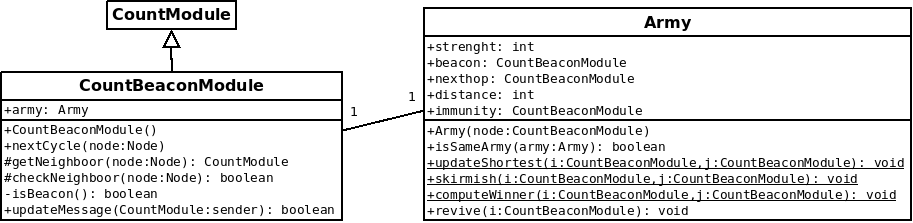
\includegraphics[height=3.5cm]{beacon_uml.png}
\caption{Diagramma UML delle classi \textsf{Army} e \textsf{CountBeaconModule}}
\label{img:beacon}
\end{figure}

La classe \textsf{CountBeaconModule} ridefinisce in particolare il metodo \textsf{nextCycle}, introducendo la computazione \textsc{beacon}, che viene effettuata con una probabilit\`a $\mathbb{P} = 0.50$. Inoltre il metodo \textsf{getNeighboor} viene ridefinito considerando il caso in cui il nodo debba inviare un nodo IC, in modo da instradarlo verso il \emph{beacon}. Il metodo \textsf{updateMessage} viene ridefinito in modo da rifiutare i messaggi $M_r$ che sono stati ricevuti da nodi che non appartengono all'esercito $A_i$ del nodo.

Per quanto riguarda la funzione \textsf{checkNeighboor} si faccia riferimento alla sezione \ref{sec:dynamic}.

La classe \textsf{Army} offre invece i metodi per gestire gli eserciti e i combattimenti fra eserciti: in particolare \textsf{skirmish} per calcolare l'esito di una schermaglia, \textsf{updateShortest} per aggiornare la distanza fra due nodi dello stesso esercito e \textsf{computeWinner} per far entrare un nodo perdente all'interno di un altro esercito pi\`u forte.

Per la funzione \textsf{revive} vale un discorso analogo a quello di \textsf{checkNeighboor} (vedi sezione \ref{sec:dynamic}).

Per far funzionare al meglio l'algoritmo \textsc{beacon} \`e inoltre necessario che venga eseguito \textsf{CountBeaconInitializer}, un inizializzatore (ovvero un'implementazione dell'interfaccia \textsf{Control} di Peersim) che permette di impostare i valori di forza ai nodi in modo casuale ideale, facendo in modo che non possano esistere due nodi con lo stesso valore di $S_i$.

\section{Reti dinamiche}
\label{sec:dynamic}

\textsc{gossipico}, come gi\`a annunciato nella sezione \ref{sec:gossipico}, \`e stato pensato per adattarsi al meglio alle situazioni di dinamicit\`a.

Pu\`o infatti succedere che all'interno della rete un nodo si disconnetta. La disconnessione pu\`o essere volontaria, nel caso in cui un nodo decida di sua spontanea volont\`a di abbandonare le rete, oppure involontaria, nel caso in cui un nodo non riesca pi\`u a connettersi ad esempio per problemi sulla rete fisica.

\textsc{gossipico} prevede che i nodi che si rendano conto di un nodo che si \`e disconnesso diano luogo ad una ``rivoluzione'' effettuando un ricalcolo, in modo da far ripartire il calcolo alla luce del nodo appena disconnesso. Il nodo effettua quindi un reset del proprio modulo \textsc{count} in modo analogo a quanto descritto in sezione \ref{sec:skirmish}. Viene poi reinizializzato l'esercito del nodo con nuovi valori (quindi un nuovo valore di $S_i = rnd()$) ed impostato il nodo come \emph{beacon} dell'esercito.

Una situazione di questo genere non risulta per\`o essere la soluzione adatta a risolvere il problema, in quanto il nodo $i$ potrebbe essere inglobato dall'esercito attualmente al potere $A_j$, andando quindi ad interrompere l'operazione di ricalcolo. Per evitare che ci\`o accada si aggiunge un nuovo campo all'esercito di ogni nodo: il campo $I_i$ che rappresenta l'\emph{Immunit\`a}:

$$I_i = j \qquad\mathrm{se}\; i \;\mathrm{risulta\;immune\;a}\; j$$

Introducendo l'\emph{Immunit\`a} si deve anche aggiornare il meccanismo delle schermaglie, prevedendo che, nel momento in cui un nodo $i$ contatta un nodo $j$, nel caso in cui sia impostato $I_i = j$ il nodo $i$ sia dichiarato automaticamente vincitore dello scontro (e viceversa).

Essendo l'\emph{Immunit\`a} un nuovo campo dell'esercito, esso viene trasmesso anche ai nuovi nodi che entrano a far parte dell'esercito.

\subsection{Implementazione}

Per implementare il supporto alle reti dinamiche, si pu\`o notare che sono presenti alcuni metodi all'interno delle classi \textsf{CountBeaconModule} e \textsf{Army} (immagine \ref{img:beacon}). In particolare \textsf{checkNeighboor} permette di controllare se tutti i vicini sono sempre up, oppure se qualche nodo si \`e disconnesso. Nel caso in cui un nodo si accorga che un nodo si \`e disconnesso esso invoca il metodo \textsf{revive} sul proprio esercito ed imposta il valore del campo \textsf{immunity} in modo da effettuare un ricalcolo.

\section{Interazione}
\label{sec:interazione}

Come si \`e potuto evincere dalle sezioni \ref{sec:count} e \ref{sec:beacon} le interazioni fra i due moduli \textsc{count} e \textsc{beacon} sono notevoli, ogni modulo funziona grazie alle informazioni raccolte dall'altro.

Le interazioni fra i due moduli possono essere riassunte nell'immagine \ref{img:interazione}
\begin{figure}[ht]
\centering
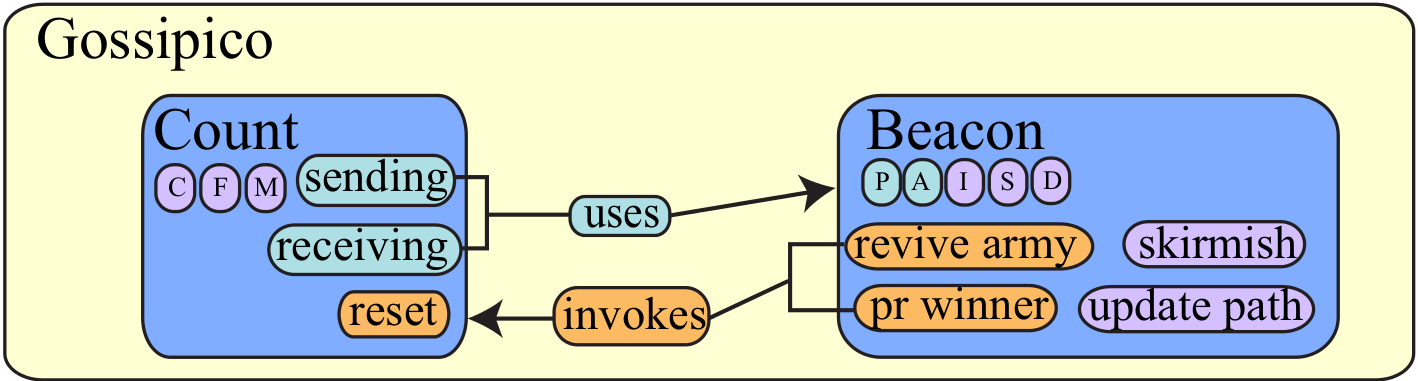
\includegraphics[height=3cm]{interazione.png}
\caption{Schema delle interazioni fra i due moduli, tratto da \cite{rif1}}
\label{img:interazione}
\end{figure}

\section{Ulteriori Classi}
\label{sec:ulteriori}

Oltre alle classi finora presentate, il software \`e stato corredato da altre classi di comodo per effettuare simulazioni pi\`u strutturate.

\subsection{Altre funzioni di aggregazione}

L'algoritmo di \textsc{count}, come gi\`a anticipato, pu\`o essere utilizzato per effettuare il calcolo di altre funzioni di aggregazione. Sono state implementate le funzioni di somma, massimo e minimo. In particolare \`e possibile scegliere la funzione da usare tramite il parametro \texttt{.func} nel file di configurazione: i valori ammissibili sono \texttt{count}, \texttt{sum}, \texttt{min} e \texttt{max}.

Per realizzare queste funzioni \`e stato sufficiente definire delle sottoclassi di \textsf{Message}, in particolare le classi \textsf{MinMessage} e \textsf{MaxMessage} (immagine \ref{img:func}), in cui si va a fare l'override del metodo \textsf{merge(m)} in modo da andare a definire quale valore deve essere conservato quando due messaggi IC si incontrano. Per quanto riguarda la funzione di somma \`e stato sufficiente impostare il valore iniziale $C_w$ del primo messaggio in attesa. Tale valore pu\`o essere impostato tramite il parametro \texttt{.value} nel file di configurazione.

\begin{figure}[ht]
\centering
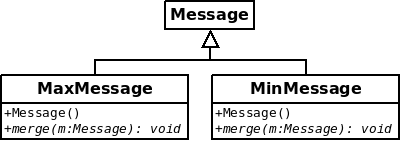
\includegraphics[height=2cm]{message_func.png}
\caption{Diagramma UML delle classi \textsf{MinMessage} e \textsf{MaxMessage}}
\label{img:func}
\end{figure}

Con \textsc{gossipico} \`e possibile effettuare anche il calcolo della funzione della media, risulta per\`o necessario ampliare il messaggio con due valori $V_w$ dove si mantiene la somma dei valori e $C_w$ dove si mantiene il conteggio dei nodi finora visti. Per implementare questa funzione non sarebbe sufficiente una classe \textsf{AvgMessage} con un campo ulteriore, ma sarebbe necessario ampliare anche la classe \textsf{CountModule} (o \textsf{CountBeaconModule}) prevedendo una nuova variabile di stato e fare l'override di tutti i metodi che coinvolgono la variabile di stato.

\subsection{Inizializzatori}

Nel caso in cui si voglia utilizzare il calcolo tramite la funzione della somma, del massimo o del minimo \`e possibile dare il valore in input tramite il parametro \texttt{.value} come presentato poco fa. In questo modo per\`o ogni nodo condivide lo stesso valore, se si volesse invece utilizzare dei valori differenti per ogni nodo si pu\`o utilizzare un inizializzatore.

Questi inizializzatori implementano l'interfaccia \textsf{Control} di Peersim e possono essere eseguiti prima dell'esecuzione della simulazione; in particolare sono disponibili i seguenti inizializzatori:
\begin{description}
\item[\textsf{LinearInitializer}] Assegna ad ogni nodo un valore che va da 0 ad $n-1$, dove $n$ \`e il numero dei nodi della rete,
\item[\textsf{PeakInitializer}] Assegna ad ogni nodo il valore 0, tranne al primo nodo a cui assegna il valore impostato dal parametro \texttt{.value} nel file di configurazione,
\item[\textsf{RandomInitializer}] Assegna valori casuali ad ogni nodo. I valori sono compresi fra gli estremi \texttt{.min} e \texttt{.max} impostati nel file di configurazione.
\end{description}
\subsection{Raccolta di statistiche}

Per la raccolta delle statistiche sull'esecuzione \`e possibile utilizzare la classe \textsf{Statistics} (implementazione di \textsf{Control}). Questa classe offre informazioni relative alla situazione della rete quali il numero dei messaggio IC, IS ed il numero dei \emph{beacon} presenti nella rete.

Inoltre visualizza a quale ciclo vengono raggiunte le 3 fasi descritte nella sezione \ref{sec:performance}. 

Nel caso di computazioni con molti cicli, se non si fosse interessati ad avere tutte le informazioni sui messaggi ad ogni ciclo, ma si \`e solamente interessati a sapere quanti cicli sono necessari all'algoritmo per convergere, si pu\`o impostare il parametro \texttt{.silent} su \texttt{true} nel file di configurazione (di default \`e su \texttt{false}).

\subsection{Debugging}

Per effettuare il debug \`e possibile usare la classe \textsf{Debugger} (implementazione di \textsf{Control}) che stampa ad ogni ciclo la situazione attuale di ogni nodo fornendo informazioni su tutto il suo stato (sia per quanto riguarda la parte \textsc{count} che la parte \textsc{beacon}).

\section{Performance}
\label{sec:performance}

Andando ad analizzare a fondo l'algoritmo si pu\`o notare che il calcolo procede in 3 fasi distinte.
\begin{enumerate}
\item Si svolge la lotta per eleggere un singolo \emph{beacon}. Il modulo \textsc{count} funziona correttamente, ma vengono invocati dei \emph{reset} ogni volta che un nodo entra a far parte di un nuovo esercito. 
\item \`E stato individuato un unico \emph{beacon}, che adesso avr\`a il compito di raccogliere tutti i messaggi IC della rete e ricombinarli. \`E possibile che avvengano altre ricombinazioni in nodi intermedi prima di arrivare direttamente al \emph{beacon}, ma noi assumiamo al caso pessimo che arrivino $n-1$ messaggi IC al \emph{beacon} dove $n$ \`e la dimensione della rete.
\item Nella rete \`e presente un singolo messaggio di tipo IC che contiene tutta l'informazione. Adesso l'informazione deve essere condivisa presso gli altri nodi attraverso i messaggi IS.
\end{enumerate}

Per poter stimare queste tre fasi introduciamo la conduttanza $\phi$ (presentata in \cite{rif12}) come misura del grado globale di connessione della rete ($0 < \phi < 1$ e vale 1 nel caso di un grafo completamente connesso). In \cite{rif12} si nota come la velocit\`a con cui un'informazione si diffonde all'interno di una rete sia proporzionale a $O(\phi^{-1} log(\mathrm{N}))$ dove N \`e il numero di nodi della rete.

Per quanto riguarda la prima e la terza fase, possiamo ricondurle facilmente alla diffusione di un'informazione su una rete, per cui vale l'approssimazione  $O(\phi^{-1} log(\mathrm{N}))$. Per la seconda fase consideriamo invece il caso pessimo in cui tutti i messaggi IC si incontrino presso il nodo \emph{beacon}; anche in questo caso il percorso pi\`u lungo verso il \emph{beacon} risulta essere dell'ordine di $O(\phi^{-1} log(\mathrm{N}))$ per cui questo limite si applica anche al secondo caso.

In media si nota che l'algoritmo \textsc{gossipico} impiega $O(log(\mathrm{N}))$ cicli per giungere alla convergenza, dimostrandosi dunque un ottimo algoritmo per il calcolo di funzioni di aggregazione, in grado di affrontare anche reti di dimensioni elevate.

\subsection{Grafici delle performance}
Per poter apprezzare a fondo \textsc{gossipico} ed in particolare l'utilit\`a del modulo \textsc{beacon} sono stati realizzati alcuni test sperimentali di cui si riportano i risultati nelle sezioni seguenti.

\subsubsection{Evoluzione del numero di messaggi IC}

Un parametro che risulta interessante analizzare \`e il numero di messaggi di tipo IC presenti ad ogni iterazione nella rete. Sappiamo infatti che l'informazione \`e stata correttamente raccolta ed aggregata quando sar\`a presente nella rete solamente un messaggio di tipo IC. Sono stati quindi monitorati il numero di messaggi IC in una simulazione con un grafo random formato da 1000 nodi.

La simulazione \`e stata realizzata utilizzando sia l'algoritmo \textsc{count} che l'algoritmo \textsc{count-beacon}.

\begin{figure}[ht]
\centering
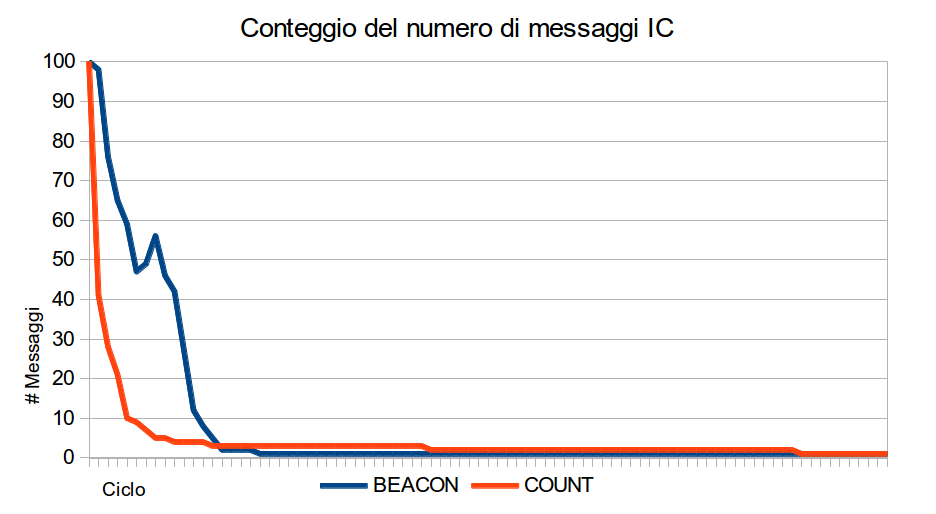
\includegraphics[height=6cm]{ic_count.png}
\caption{Grafico che rappresenta il numero di messaggi IC presenti nella rete}
\label{img:graph_count}
\end{figure}

I risultati sono mostrati nell'immagine \ref{img:graph_count}, si pu\`o notare come il numero dei messaggi decresca in entrambi i casi, ma decresce in modo pi\`u immediato il numero nel caso dell'algoritmo \textsc{count}. 

Questo fenomeno deriva dal fatto che l'algoritmo \textsc{beacon} fa effettuare dei \emph{reset} ai nodi che sono stati appena inseriti in un nuovo esercito. Quando si effettua un \emph{reset} il nodo viene reimpostato con il messaggio $M_w$ su $\{1, 1, 1\}$ che contribuisce ad aumentare il conteggio dei messaggi IC.

Se si osserva attentamente il grafico si pu\`o notare che, correttamente, l'utilizzo del modulo \textsc{beacon} velocizza la convergenza (che in questo caso viene raggiunta in circa 50 cicli), mentre l'algoritmo \textsc{count} porta ad uno stato in cui sono presenti pochi messaggi IC che viaggiano in modo casuale nella rete. Questa situazione permane per molti cicli fino a quando i messaggi IC non si incontrano presso un singolo nodo (in questo caso all'incirca dopo 600 cicli).

\subsubsection{Velocit\`a di convergenza}

Un altro parametro fondamentale da misurare risulta essere il numero di cicli necessari all'algoritmo per raccogliere tutta l'informazione e distribuirla a tutti i nodi.

Sono stati effettuati vari test variando algoritmo e topologia di rete:
\begin{itemize}
\item Algoritmo \textsc{count} con grafi random.
\item Algoritmo \textsc{count-beacon} con grafi random.
\item Algoritmo \textsc{count-beacon} con grafi \emph{small-world} di Watts and Strogatz.
\item Algoritmo \textsc{count-beacon} con grafi \emph{scale-free} di Barabasi-Albert.
\end{itemize}

Sono state dapprima effettuate simulazioni su reti di piccole dimensioni (immagine \ref{img:speed_low}) in cui si pu\`o notare come, gi\`a su reti di dimensioni superiori a 100 nodi, l'aggiunta del modulo \textsc{beacon} velocizza notevolmente il calcolo.

\begin{figure}[ht]
\centering
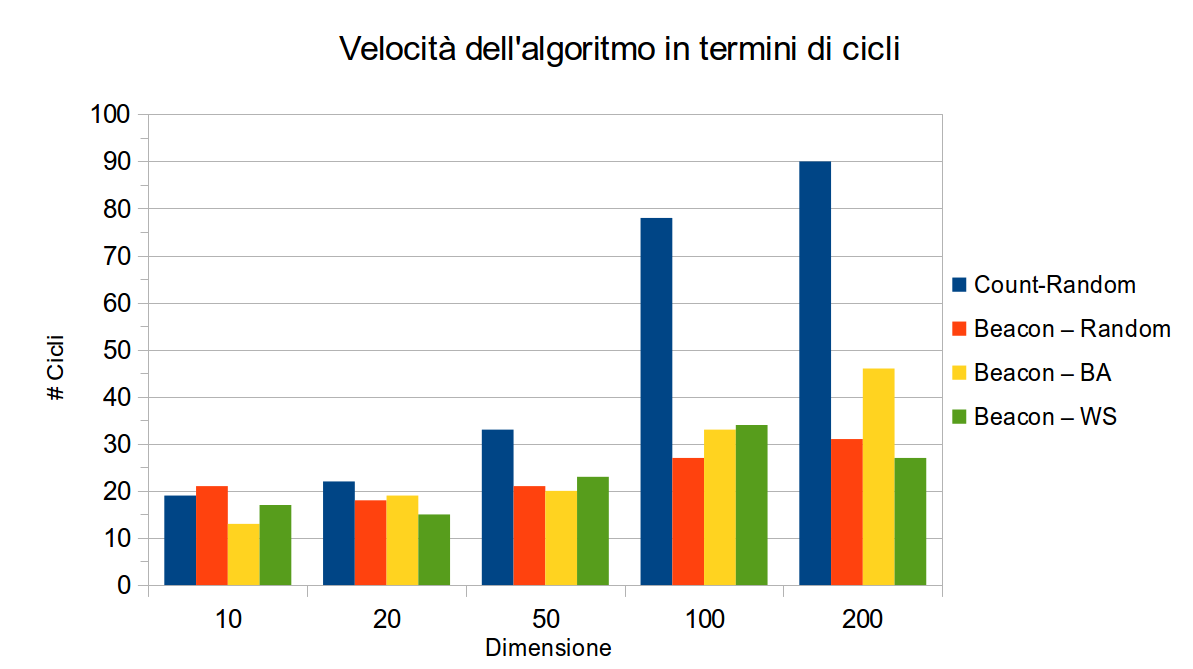
\includegraphics[height=6cm]{speed_low.png}
\caption{Grafico che rappresenta la velocit\`a di convergenza su reti di piccole dimensioni}
\label{img:speed_low}
\end{figure}

I risultati davvero interessanti si ottengono per\`o quando si effettuano simulazioni su reti di medie o grandi dimensioni (immagine \ref{img:speed}), in cui il modulo \textsc{beacon} permette un notevole miglioramento delle performance. Si noti che nell'immagine \ref{img:speed} la scala sull'asse $y$ risulta essere logaritmica in modo da rappresentare al meglio il miglioramento introdotto.

\begin{figure}[ht]
\centering
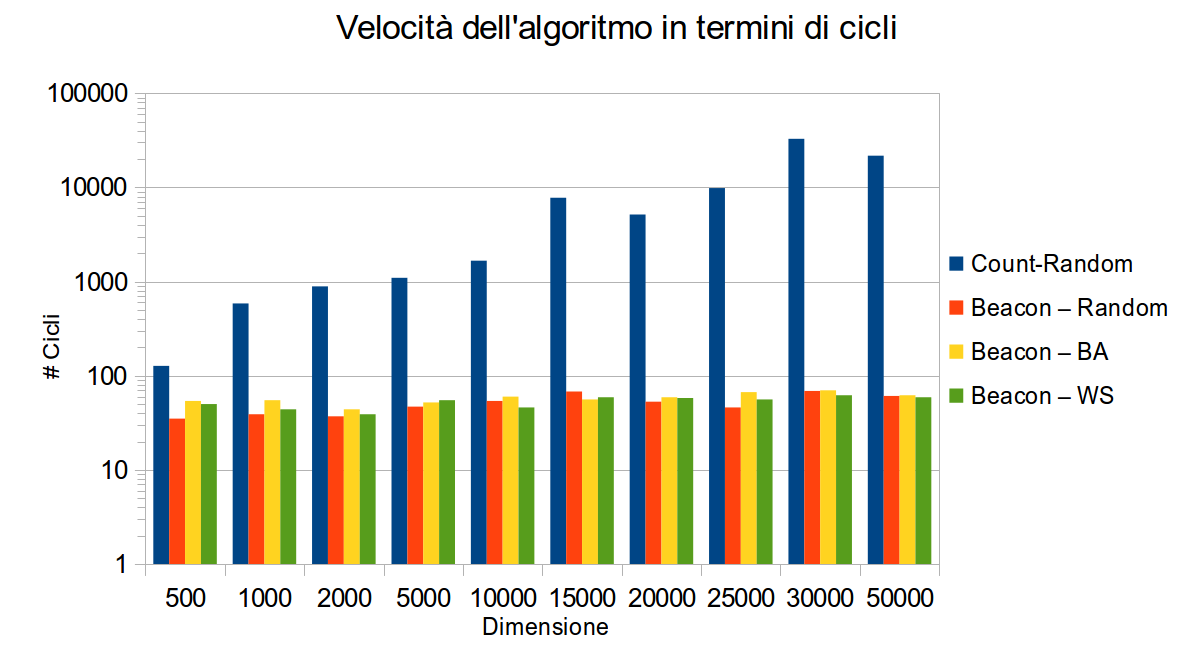
\includegraphics[height=6cm]{speed.png}
\caption{Grafico che rappresenta la velocit\`a di convergenza su reti di medie e grandi dimensioni}
\label{img:speed}
\end{figure}

\subsubsection{Evoluzione in caso di disconnessione di nodi}

Un'ultima simulazione che risulta molto interessante da analizzare \`e quella che rappresenta l'evoluzione della rete nel caso in cui un nodo si disconnetta.

In particolare si va ad analizzare la stima della dimensione della rete calcolata nel modo seguente:
\begin{equation}\label{eq:stima}
S = \frac{\sum\limits_{i=1}^{k} M_i.C}{k}
\end{equation}

Dove $k = Network.size()$. 

Nei grafici nell'immagine \ref{img:dyna} si va ad analizzare la differenza fra la stima calcolata e la dimensione effettiva della rete.

\begin{figure}[ht]
\centering
\begin{subfigure}[b]{1\textwidth}
	\centering
	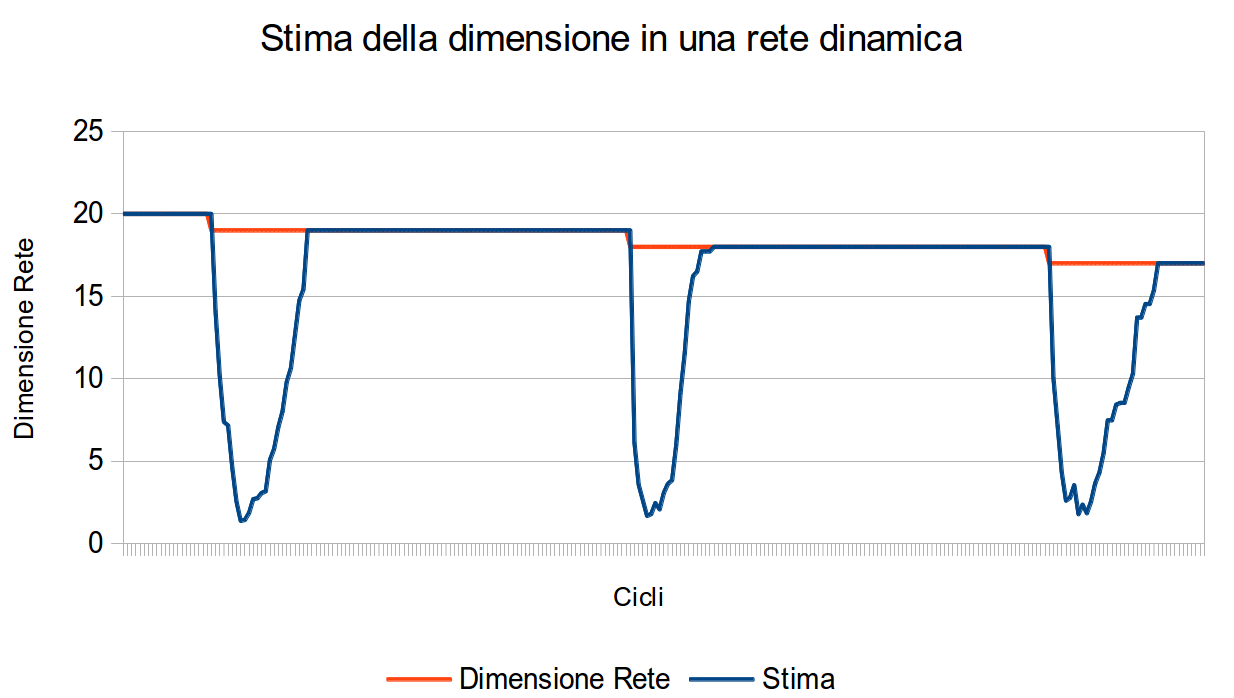
\includegraphics[height=6cm]{dynamic.png}
	\caption{Disconnessioni distanti}	
	\label{img:dyna_a}
	\vspace{1cm}
\end{subfigure}
\begin{subfigure}[b]{1\textwidth}
	\centering
	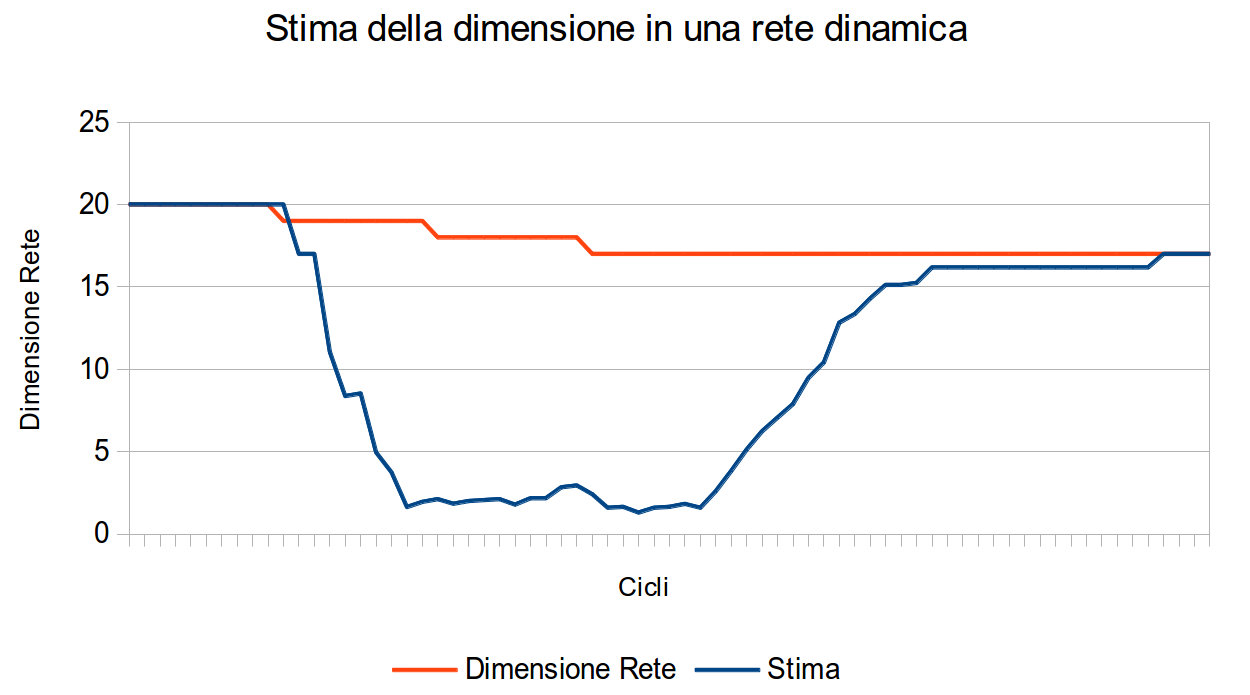
\includegraphics[height=6cm]{dynamic2.png}
	\caption{Disconnessioni ravvicinate}	
	\label{img:dyna_b}
\end{subfigure}
\caption{Grafico che rappresenta la stima della dimensione della rete in condizioni di dinamicit\`a}
\label{img:dyna}
\end{figure}

Nel grafico in immagine \ref{img:dyna_a} le disconnessioni sono distanziate nel tempo, per cui si nota chiaramente che l'algoritmo riesce a raggiungere senza problemi il valore di dimensione della rete effettivo.

Nel grafico in immagine \ref{img:dyna_b} sono invece presenti tre disconnessioni ravvicinate. Si nota come la rete si adatti a queste disconnessioni: viene fatto partire un riconteggio e la stima tende a riallinearsi al valore effettivo; in prossimit\`a dell'ultima disconnessione viene fatto partire un nuovo riconteggio (si noti come la linea blu nella parte centrale decresce leggermente) e l'algoritmo riesce comunque ad approssimare comunque l'effettiva dimensione della rete.

\paragraph{Utilizzo di una funzione logistica}
Si noti come in entrambi le figure \ref{img:dyna_a} e \ref{img:dyna_b} la stima del calcolo precipita bruscamente dopo ogni disconnessione. Per avere delle stime pi\`u precise, invece di considerare la formula \ref{eq:stima} si potrebbe utilizzare la formula seguente:
\begin{equation}\label{eq:stima_log}
X = \left\{
\begin{array}{ll}
(1 - f(t)) X_{old} \;+\; f(t) C_s & \mbox{se}\; C_s < X_{old}\\
C_s & \mbox{se}\; C_s \geq X_{old}
\end{array}
\right.
\end{equation}

Dove il valore $X_{old}$ rappresenta il vecchio valore conservato dal nodo prima del riconteggio e $f(t)$ risulta essere la funzione logistica seguente:
\begin{equation}\label{eq:logistica}
f(t) = \frac{1}{1 + e^{-t + 2D + 5}}
\end{equation}
Dove $D$ rappresenta la distanza verso il beacon, e il valore $t$ rappresenta il numero di cicli in cui un nodo ha generato lo stesso messaggio IS (quindi un numero che cresce al procedere della simulazione), in modo da poter shiftare la stima da $X_{old}$ verso il nuovo $C_s$.

\section{User guide}
\label{sec:guide}

La simulazione \`e stata realizzata in Java utilizzando il simulatore Peersim ed \`e stata corredata di un file \textbf{ant} (il file \texttt{build.xml}) che offre dei target per automatizzare il processo di compilazione e di esecuzione del software.

Per funzionare, la simulazione ha bisogno di un file di configurazione in input da cui poter caricare la configurazione della rete (numero di nodi, numero di link, protocolli da utilizzare, etc...). Alcuni esempi di file di configurazione possono essere trovati all'interno della cartella \texttt{example/}.

Per compilare la simulazione \`e necessario posizionarsi all'interno della directory dove \`e contenuto il software ed invocare da terminale il comando

\begin{lstlisting}[basicstyle=\ttfamily]
ant build
\end{lstlisting}

che provveder\`a ad invocare il compilatore \texttt{javac} per compilare i sorgenti presenti all'interno della cartella \texttt{src/}, i file \texttt{.class} generati si troveranno all'interno della cartella \texttt{bin/}. 

Per pulire la cartella \texttt{bin/} al fine di avere un ambiente pulito per poter effettuare una nuova compilazione \`e possibile utilizzare il target
\begin{lstlisting}[basicstyle=\ttfamily]
ant clean
\end{lstlisting}

\`E infine possibile generare un file \texttt{jar} contenente tutti i file compilati e tutte le librerie necessarie all'esecuzione. Per farlo \`e sufficiente invocare il target
\begin{lstlisting}[basicstyle=\ttfamily]
ant jar
\end{lstlisting}
Verr\`a generato un file chiamato \texttt{p2p\_final.jar} all'interno della cartella principale del software.
Per avviare il file \texttt{jar} \`e necessario invocare il comando
\begin{lstlisting}[basicstyle=\ttfamily]
java -jar p2p_final.jar [file di configurazione]
\end{lstlisting}

\subsection{Documentazione}

Al fine di rendere il codice sorgente pi\`u comprensibile, il software \`e stato corredato di documentazione. In particolare tutte le parti del codice sorgente che potrebbero risultare di difficile comprensione sono state commentate. Inoltre ogni funzione e classe del software \`e stata documentata con il formato \textsf {javadoc}, la documentazione generata pu\`o essere visionata all'interno della cartella \textsf{doc/} e pu\`o essere rigenerata utilizzando il comando
\begin{lstlisting}[basicstyle=\ttfamily]
ant javadoc
\end{lstlisting}

Per una comprensione organica del software si consiglia la lettura della seguente relazione nella sua interezza. La presente relazione viene rilasciata in Pdf ed in \LaTeX\ e pu\`o essere visionata all'interno della cartella \texttt{doc/tex/}.

\subsection{Avvio della simulazione}

Una volta compilato il software \`e possibile invocarlo tramite il comando
\begin{lstlisting}[basicstyle=\ttfamily]
ant Execute [-Dfile=nomefile]
\end{lstlisting}

Con \texttt{-Dfile=nomefile} \`e possibile impostare il file di configurazione da usare. Per effettuare alcune computazioni di esempio \`e quindi sufficiente impostare \texttt{-Dfile=example/<nomefile.conf>}, eseguendo alcuni dei files di esempio gi\`a predisposti all'interno della cartella \texttt{example}.

I nomi dei files contenuti nella cartella \texttt{example} permettono di comprendere facilmente quali sono le configurazioni impostate. Sono stati predisposti calcoli solamente \textsc{count} oppure \textsc{count-beacon}, con grafi random, small-world e scale-free. Inoltre sono stati predisposti esempi con debugger attivato ed altri esempi in cui si calcolano altre funzioni (massimo, somma, etc...).

Se la struttura dei file di configurazione non fosse chiara \`e possibile visionare il file \textsf{example.conf} che contiene tutti i commenti necessari a comprendere le impostazioni possibili.

\appendix
\section{Codice Sorgente}

Di seguito \`e presente il codice sorgente dell'applicazione diviso per classi. Sono presenti i commenti prima di ogni classe, metodo e campo nello stile Javadoc. Sono inoltre presenti i commenti all'interno dei punti critici del codice per comprendere a meglio i punti pi\`u delicati.

\subsection{Classi relative a COUNT}

\subsubsection{Classe \textsf{CountModule}}

\lstinputlisting{src/CountModule.java}

\subsubsection{Classe \textsf{Message}}

\lstinputlisting{src/Message.java}

\subsection{Classi relative a BEACON}

\subsubsection{Classe \textsf{CountBeaconModule}}

\lstinputlisting{src/CountBeaconModule.java}

\subsubsection{Classe \textsf{Army}}

\lstinputlisting{src/Army.java}

\subsection{Classi di Inizializzatori}

\subsubsection{Classe \textsf{CountBeaconInitializer}}

\lstinputlisting{src/CountBeaconInitializer.java}

\subsubsection{Classe \textsf{RandomInitializer}}

\lstinputlisting{src/RandomInitializer.java}

\subsubsection{Classe \textsf{PeakInitializer}}

\lstinputlisting{src/PeakInitializer.java}

\subsubsection{Classe \textsf{LinearInitializer}}

\lstinputlisting{src/LinearInitializer.java}

\newpage

\subsection{Sottoclassi di \textsf{Message}}

\subsubsection{Classe \textsf{MaxMessage}}

\lstinputlisting{src/MaxMessage.java}

\subsubsection{Classe \textsf{MinMessage}}

\lstinputlisting{src/MinMessage.java}

\subsection{Classi di Osservatori}

\subsubsection{Classe \textsf{Debugger}}

\lstinputlisting{src/Debugger.java}

\subsubsection{Classe \textsf{Statistics}}

\lstinputlisting{src/Statistics.java}

\newpage

\begin{thebibliography}{100}

\bibitem{rif1} van de Bovenkamp, Ruud, Fernando Kuipers, and Piet Van Mieghem. "Gossip-based counting in dynamic networks." NETWORKING 2012. Springer Berlin Heidelberg, 2012. 404-417.

\bibitem{rif12} Giakkoupis, George. "Tight bounds for rumor spreading in graphs of a given conductance." Leibniz International Proceedings in Informatics (LIPIcs) series 9 (2011): 57-68.

\bibitem{rif2} Peersim Simulator, \url{http://peersim.sourceforge.net/}


\end{thebibliography}

\end{document}
